% vim:encoding=utf8 ft=tex sts=2 sw=2 et:
% Copyright (c) 2009 Jaroslaw Koszuk
%
% $Id$

\documentclass{jacsart}

\usepackage[utf8]{inputenc}
\usepackage[T1]{fontenc}
\usepackage{graphicx}
\usepackage{amsthm}
\usepackage{txfonts}

\newtheorem{definition}{Definition}
\newtheorem{theorem}[definition]{Theorem}
\newtheorem{corollary}[definition]{Corollary}
\newtheorem{proposition}[definition]{Proposition}
\newtheorem{example}[definition]{Example}


\title{Title of the paper submitted to the Journal of Applied Computer
  Science\footnote{put a footnote to the title if necessary}}
\headtitle{Title of the paper submitted to JACS\dots}
\author{Author One\inst{1}, Author Two\inst{1,2}}
\headauthor{A. One, A. Two}
\affiliation{%
  \inst{1}Name of the Unit represented (e.g. Your University)\\
  Faculty/Department/Office Name\\
  Postal Addres with the zip-code\\
  yourid@your.mail.server
  \andinst
  \inst{2}Name of the Unit represented (e.g. Your University)\\
  Faculty/Department/Office Name\\
  Postal Addres with the zip-code\\
  yourid@your.mail.server}
\keywords{keyword 1, keyword 2, keyword 3, keyword, keyword, keyword, keyword, keyword, keyword}

\begin{document}
\maketitle

\begin{abstract}
Each paper should be followed by a compact abstract which points to the main
scopes and the results obtained by the paper. The abstract should be written
with the Times New Roman font, 10 pt, justified, and with the 1cm margin both
left and right side with respect  to the margin of the paper. The abstract should not contain any formulas or references, and should not exceed 200 words. 
\end{abstract}

\section{Title of section}
\indent Journal of Applied Computer Science publishes original papers only. Full
papers not exceeding 22 standard pages (30 lines $\times$ 60 characters), should be
submitted electronically (preferably by e-mail), or on CD. They will not be returned except for
editorial reasons.\\
\indent Contributions should be written in good English and prepared in \LaTeX. The Authors are strongly
encouraged to follow the \LaTeX{} {\tt jacsart.cls} and BiBTeX {\tt
aiaa-jacs.bst} styles included to this template, as far as published at:\newline
{\tt http://www.jacs.ics.p.lodz.pl}.\\
\indent Illustrations (with captions), drawings, tables, diagrams and equations should be
incorporated in the text and numbered consecutively. Mathematical symbols should
be typeset using the math mode of \LaTeX. The references should be
enumerated in order of appearing in text, and formatted as shown in
Section~\ref{bib}, p.~\pageref{bib}, preferably using the BiBTeX style {\tt
aiaa-jacs.bst}. 


Lorem ipsum dolor sit amet, consectetur adipiscing elit. Nam elit. Etiam
hendrerit. Nulla arcu. Etiam convallis, lectus in feugiat consequat, tortor
orci laoreet erat, in varius leo nisi pharetra orci. Sed arcu elit, semper
pulvinar, tempor vel, rhoncus in, risus. Nunc dignissim massa id dui. Aenean
viverra, odio ac tincidunt adipiscing, augue ligula faucibus velit, ac
sollicitudin lacus tellus sed elit. 

\begin{definition} \label{label-of-definition}
The text of your definition goes here
\end{definition}

\begin{theorem} \label{label-of-theorem}
The text of your theorem goes here
\end{theorem}

\begin{proposition} \label{label-of-proposition}
The text of your proposition goes here
\end{proposition}

\begin{corollary} \label{label-of-corollary}
The text of your corollary goes here
\end{corollary}

\begin{proof} \label{label-of-proof}
The text of your proof goes here
\end{proof}


Quisque ultricies\footnote{An example of footnote} tortor non elit. Nunc vestibulum. Donec libero. Sed id quam
auctor odio semper rutrum. Proin convallis neque quis nisl. Praesent tempor
est vel urna. Etiam bibendum ipsum pellentesque felis. Phasellus et sapien
quis sem tincidunt lobortis. Quisque ultricies tincidunt justo. Maecenas at
nibh a urna condimentum fermentum. Duis tempor, ante vel rhoncus fermentum,
velit dui dignissim odio, ut suscipit quam massa eu velit.

Sed placerat ultrices urna. Sed tincidunt eleifend nibh. In scelerisque dictum
enim. Duis sit amet lectus ut lorem hendrerit sodales. 

\begin{figure}[!t] %figures should be placed at the top of the page
\centering
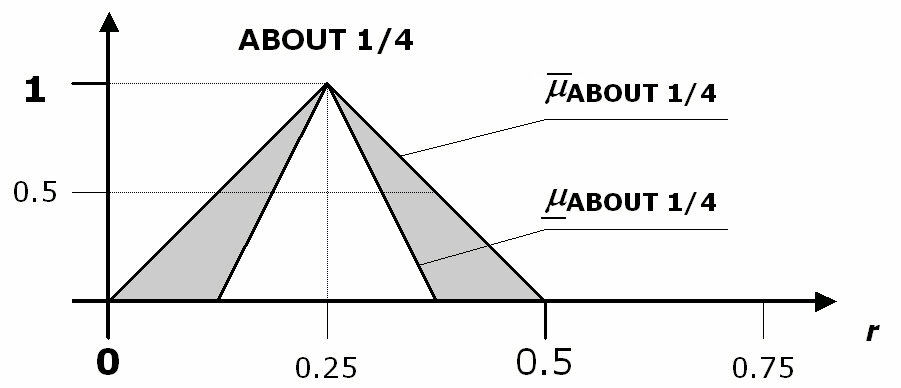
\includegraphics[width=0.9\textwidth]{5figivfq}
\caption{This is caption of the figure}
\label{label-of-figure-1}
\end{figure}

Aliquam porttitor, lectus at gravida posuere, purus est pellentesque odio,
interdum auctor pede orci a diam. Pellentesque tincidunt tincidunt sem.
Curabitur ut enim sit amet turpis cursus adipiscing. 

\subsection{The title of subsection 1}
Phasellus tincidunt.
Praesent sit amet erat. Maecenas volutpat vehicula dui. Maecenas ligula urna,
cursus ac, egestas in, bibendum at, tellus. In posuere. Nullam orci sem,
hendrerit lobortis, facilisis eget, accumsan non, ipsum. Integer euismod.
Class aptent taciti sociosqu ad litora torquent per conubia nostra, per
inceptos himenaeos. In molestie velit ut purus. Suspendisse id erat. Phasellus
bibendum purus egestas sapien. 

\begin{equation} \label{label-of-equation-1}
  e^{i \pi} + 1 = 0
\end{equation}

Donec rhoncus turpis in tellus. Integer tellus. Etiam in lectus ac nunc
placerat interdum. Sed tincidunt porta enim. Aenean at massa a nisi volutpat
bibendum. Vivamus purus. 

\begin{eqnarray}
\mu_3(x) = \left\{ 
\begin{array}{cc}
      {x-3 \over 7}, & \mbox{if $3 \leq x \leq 10$} \\
      0, & \mbox{otherwise}
\end{array}
\right.
\end{eqnarray}

Praesent nec leo. Pellentesque sodales arcu ac quam.
Aliquam elit leo, lobortis eget, tincidunt sed, consequat at, elit. Aenean ut
diam. Nulla id nibh nec odio eleifend luctus. Maecenas orci arcu, fermentum
sed, placerat a, aliquet nec, felis.

\subsection{The title of subsection 2}
Donec risus. Aliquam vel nibh. Nulla gravida accumsan quam. Suspendisse
lacinia ligula ut orci. Donec ligula erat, pellentesque sed, fermentum a,
viverra euismod, diam. Integer consectetur, leo eu bibendum iaculis, libero
felis porttitor tortor, nec facilisis augue enim eget ligula. Phasellus ac leo
eu augue sagittis pulvinar. Sed feugiat. Nullam lorem est, sodales sed,
sagittis vitae, viverra sed, magna. Nulla urna magna, volutpat vitae,
fermentum id, ultrices sed, pede. Pellentesque et libero.

\subsubsection{The title of subsubsection} 
Mauris semper quam
eget massa. Nam turpis orci, sollicitudin ac, suscipit et, auctor sit amet,
lacus. Integer ut justo nec ligula rutrum bibendum. Cras vehicula nisl id
magna. Suspendisse ultricies varius mauris.
\begin{eqnarray}
CL(\mbox{$x$ is $l_i$ {\sc and} $l_j$}) = \mu_{S_i \cap
S_j}(x) = & \nonumber \\
= \left[\min\{\underline\mu_{S_i}(x), \underline\mu_{S_j}(x)\},\right. & \left. \min\{\overline\mu_{S_i}(x), \overline\mu_{S_j}(x)\}\right] 
\end{eqnarray}


\paragraph{The title of paragraph}
Integer commodo ipsum vitae enim. Morbi mollis nunc suscipit nisl.
Class aptent taciti sociosqu ad litora torquent per conubia nostra, per
inceptos himenaeos. Nam urna lacus, placerat posuere, dapibus eget, gravida
at, lorem. Aliquam nec justo eu dui semper fringilla. 

\subparagraph{The title of subparagraph}
Aliquam vitae urna.

Morbi mattis consectetur ante. Ut ante massa, vestibulum ut, accumsan ac,
convallis quis, orci. Pellentesque at ipsum vitae quam laoreet tristique. Cras
vel nunc. Nulla facilisi. Aliquam erat volutpat. Cras ipsum
odio, gravida sed, aliquet eget, gravida at, pede. Nulla eros tellus, ornare
in, ultrices porttitor, ultricies eget, justo. Etiam porttitor rutrum erat.
Donec quam.

\begin{table}[!t]
\caption{The caption of the table} 
\centering
\begin{tabular}{ | l | l | l | p{5cm} |}
\hline
\bf Day & \bf Min Temp & \bf  Max Temp & \bf Summary \\ \hline
Monday & 11C & 22C & A clear day with lots of sunshine.  
However, the strong breeze will bring down the temperatures. \\ \hline
Tuesday & 9C & 19C & Cloudy with rain, across many northern regions. Clear spells 
across most of Scotland and Northern Ireland, 
but rain reaching the far northwest. \\ \hline
Wednesday & 10C & 21C & Rain will still linger for the morning. 
Conditions will improve by early afternoon and continue 
throughout the evening. \\
\hline
\end{tabular}
\label{label-of-table}
\end{table}

 

\section{Conclusions}
Ut purus. Nullam facilisis porttitor enim. Vestibulum nulla massa, ultricies
sed, molestie luctus, imperdiet eget, mi. \\
\indent Integer commodo ipsum vitae enim. Morbi mollis nunc suscipit nisl.
Class aptent taciti sociosqu ad litora torquent per conubia nostra, per
inceptos himenaeos. Nam urna lacus, placerat posuere, dapibus eget, gravida
at, lorem. Aliquam nec justo eu dui semper fringilla. Aliquam vitae urna.
Morbi mattis consectetur ante. Ut ante massa, vestibulum ut, accumsan ac,
convallis quis, orci. Pellentesque at ipsum vitae quam laoreet tristique. Cras
vel nunc. Nulla facilisi.\\
\indent Pellentesque fringilla nulla vitae metus varius faucibus. Fusce aliquet
vehicula risus. Donec pulvinar viverra lectus. Nam tristique. Nulla malesuada
metus nec purus. Ut aliquam diam. Phasellus eu dui vel ipsum aliquet
vestibulum. Quisque ullamcorper, ligula in placerat imperdiet, risus risus
malesuada dolor, ut scelerisque ipsum nisi eu urna. Mauris bibendum tortor
condimentum mauris.  


\subsection{Some notes on references}\label{bib}
The references should be formatted using the BiBTeX program and the\newline {\tt
aiaa-jacs.bst} style. Here are examples of citing: \cite{sambuc75}, \cite{chiclana04,
bartkiewicz00, atanassov83}. 

%%%%%%%%%% USE ____BIBTEX____ TO GENERATE YOUR REFERENCES 
%%%%%%%%%%% PLEASE UNCOMMENT THE TWO FOLLOWING LINES 

%%%%%%%%%% please DO NOT use the \bibitem command %%%%%%%%%%%%
%%%%%%%%%% or the {thebibliograhy} environment    %%%%%%%%%%%% 

\bibliography{references-jacs} % or any of your reference files with entries 
\bibliographystyle{aiaa-jacs}  



\end{document}
